\documentclass[twocolumn]{styles/IEEEtran}

\usepackage{graphicx,epsfig, url}
\usepackage{times}
\usepackage{color,ifthen}

\newcommand{\sq}[2]{%
    \definecolor{thiscol}{gray}{.#2}%
        \ifthenelse{#2<50}%
            {\color{white}}%
            {\color{black}}%
        \colorbox{thiscol}{\makebox[2em]{#1}}}

%\topmargin -1.5cm

\begin{document}

\begin{figure}
 \begin{center}
 \includegraphics[width=3in]{fig/JPLB4.eps}
 \includegraphics[width=3in]{fig/JPLAFTER.eps}
\caption{An example of treatment learning results}
 \label{tab:tech_example}

 \end{center}
 \end{figure}


\newpage

\begin{figure*}
\begin{minipage}{.65\linewidth}
 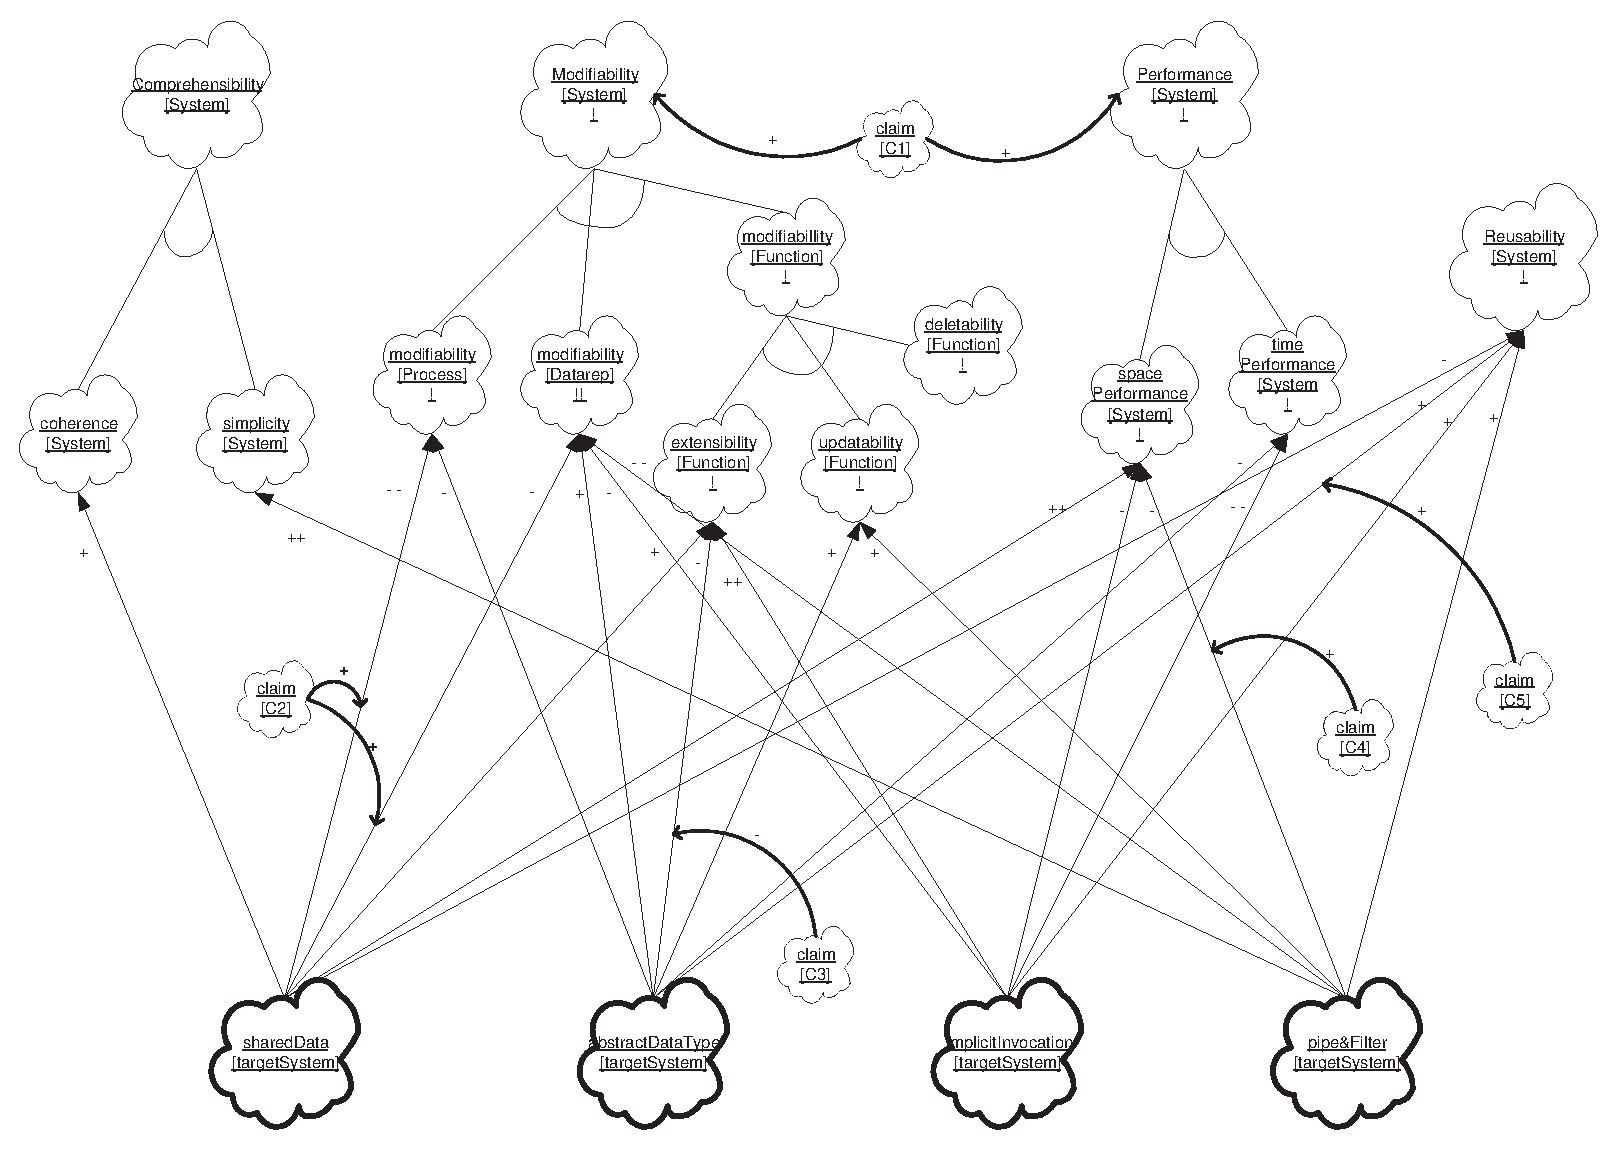
\includegraphics[width=7in]{fig/sig.eps}
 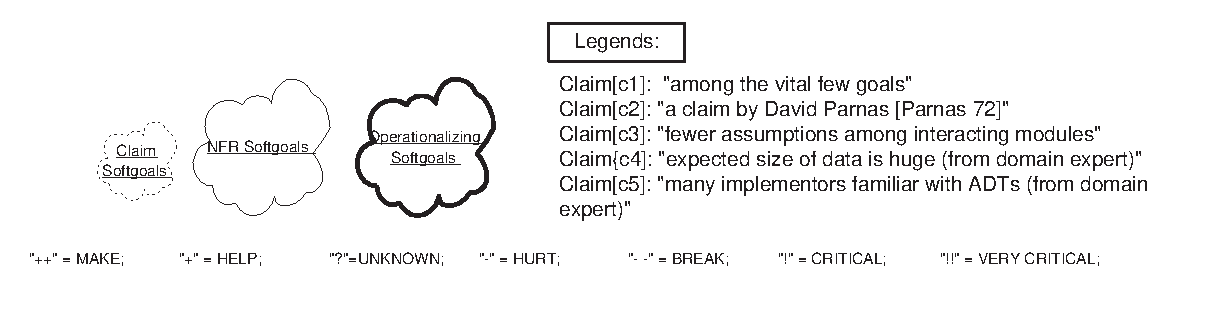
\includegraphics[width=7in]{fig/arch_def_graph_legend.eps}
\end{minipage}\hfill

\caption{KWIC framework}
\label{fig:arch_def}

\end{figure*}

\newpage
%\input{tar2}
 \begin{table}[h]
 \begin{center}
 \begin{small}
 \begin{tabular}[t]{|c|cccccc|} \hline
 & \multicolumn{6}{c|}{Benefit} \\ 
 Cost	& vvlow 	& vlow 	& low 	& high 	& vhigh	& vvhigh \\ \hline
 zero 	& 26 	& 17 	& 10 	& 5 	& 2 	& 1 \\ 
 one 	& 28 	& 19 	& 12 	& 7 	& 4 	& 3 \\ 
 two 	& 30 	& 21	& 14 	& 9 	& 8 	& 6 \\ 
 three 	& 32 	& 23 	& 16 	& 15 	& 13 	& 11 \\ 
 four 	& 34 	& 25 	& 24 	& 22 	& 20 	& 18 \\ 
 five 	& 36 	& 35 	& 33 	& 31 	& 29 	& 27 \\ \hline
 \end{tabular}
 \end{small}
 \end{center}
 \caption{class rankings for KWIC framework}
 \label{tab:arch_def_rigorous_rank1}
 \end{table}

\newpage

%\section{Case Studies}

\begin{figure}[h]
\begin{center}
\begin{footnotesize}
 \begin{tabular}[t]{|c|c|c|} \hline
 {\verb1<combine_logic>1}	& {\verb1<op>1} 	& {\verb1<arithmetic[op]>1}\\ \hline
 {\sl all\_of}		& {\verb1rand1}	& minimum \\
 {\sl any\_of}		& {\verb1rany1}	& summation \\
 {\sl any\_one\_of}		& {\verb1ror1}	& maximum \\ \hline
 {\verb1<contribution>1}	& {\verb1<value>1} 		& {\verb1<arithmetic>1}\\ 
 			& {\verb1[contribution]1} 		& {\verb1[contribution]1}\\ \hline
 {\sl helped}		& mean=1.4			& multiply \\
 {\sl made}		& mean=1.8			& multiply \\
 {\sl unhurt}		& mean=0.6			& multiply \\
 {\sl unbroken}		& mean=0.2			& multiply \\ \hline
 {\verb1<priority>1}		& {\verb1<value>1} 		& {\verb1<arithmetic>1}\\
 			& {\verb1[priority]1} 		& {\verb1[priority]1}\\ \hline
 {\sl veryCritical}		& mean=2.0			& multiply \\
 {\sl critical}		& mean=1.5			& multiply \\
 {\sl normal}		& mean=1.0			& multiply \\ \hline
 {\verb1<softgoal>1}	& {\verb1<softgoalType>1} 		& {\verb1<cost>1}	\\
 			& {\verb1[softgoal]1} 		&  {\verb1[softgoalType]1}  \\ \hline
 {\sl operationalizing}	&  any type			& 1\\ 
 {\sl softgoal	}	&  				& \\ \hline
 \end{tabular}
\end{footnotesize}
\end{center}
 \caption{Settings for KWIC framework}
\label{fig:arch_def_rigorous_config}
\end{figure} 

\begin{figure}[h]
\begin{center}
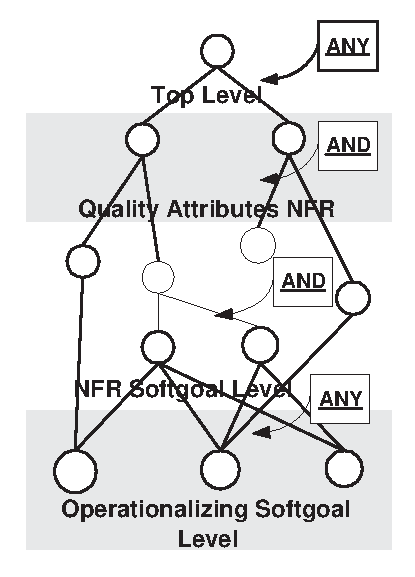
\includegraphics[width=1.5in]{fig/arch_def_rigorous_graph.eps}

\end{center}
\caption{logic configuration for rigorous quality assurance scheme}
\label{fig:arch_def_rigorous_graph}
\end{figure}

\begin{table}[h]
 \begin{footnotesize} 
 \begin{center}
 \begin{tabular}[t]{|c|c@{ }c@{ }c@{ }c@{ }c@{ }c|c|} \hline
 & \multicolumn{6}{c|}{Benefit} & \\ 
 Cost	& $<5.5$		&$<11$		& $<16.5$	& $<22$		& $<27.5$	& $<32$ 		& 	\\ \hline
0	&	 	& 	 	& 	 	& 	 	& 	 	& 	 	& 	 \\
1	& \sq{3.86}{96} 	& 	 	& 	 	& 	 	& 	 	& 	 	& \sq{3.86}{96} \\
2	& \sq{32.9}{67} 	& \sq{0.27}{99} 	& 	 	& 	 	& 	 	& 	 	& \sq{33.17}{66} \\
3	& \sq{10.01}{89} 	& \sq{3.49}{96} 	& \sq{0.02}{99} 	& 	 	& 	 	& 	 	& \sq{13.52}{86} \\
4	& \sq{6.66}{93} 	& \sq{22.68}{77} 	& \sq{5.88}{94} 	& \sq{0.45}{99} 	& \sq{0.02}{99} 	& 	 	& \sq{35.69}{64} \\
5	& \sq{1.06}{98} 	& \sq{6.74}{93} 	& \sq{4.94}{95} 	& \sq{0.95}{99} 	& \sq{0.07}{99} 	& 	 	& \sq{13.76}{86} \\ \hline
total	& \sq{54.49}{45} 	& \sq{33.18}{66} 	& \sq{10.84}{89} 	& \sq{1.4}{98} 	& \sq{0.09}{99} 	& 	 	& \sq{100}{2} \\ \hline
 \end{tabular}
 \end{center}
 \end{footnotesize}
 \caption{\textbf{Round 1} Percentage distributions of $benefit$s and $cost$s seen in 10,000 runs of fig \ref{fig:arch_def_rigorous_graph}; no treatment}
 \label{arch_def_rigorous_better4_1}


 \begin{footnotesize} 
 \begin{center}
 \begin{tabular}[t]{|c|c@{ }c@{ }c@{ }c@{ }c@{ }c|c|} \hline
 & \multicolumn{6}{c|}{Benefit} & \\ 
 Cost	& $<5.5$		&$<11$		& $<16.5$	& $<22$		& $<27.5$	& $<32$ 		& 	\\ \hline
0	&	 	& 	 	& 	 	& 	 	& 	 	& 	 	& 	 \\
1	&	 	& 	 	& 	 	& 	 	& 	 	& 	 	& 	 \\
2	&\sq{27.84}{72} 	& 	 	& 	 	& 	 	& 	 	& 	 	& \sq{27.84}{72} \\
3	&\sq{10.71}{89} 	& \sq{7.05}{92} 	& \sq{0.28}{99} 	& 	 	& 	 	& 	 	& \sq{18.04}{81} \\
4	&\sq{4.26}{95} 	& \sq{8.89}{91} 	& \sq{1.7}{98} 	& \sq{0.11}{99} 	& \sq{0.01}{99} 	& 	 	& \sq{14.97}{85} \\
5	&\sq{2.83}{97} 	& \sq{19.2}{80} 	& \sq{14.68}{85} 	& \sq{2.24}{97} 	& \sq{0.19}{99} 	& \sq{0.01}{99} 	& \sq{39.15}{60} \\ \hline
total	&\sq{45.64}{54} 	& \sq{35.14}{64} 	& \sq{16.66}{83} 	& \sq{2.35}{97} 	& \sq{0.2}{99} 	& \sq{0.01}{99} 	& \sq{100}{2} \\ \hline
 \end{tabular}
 \end{center}
 \end{footnotesize}
 \caption{\textbf{Round 2} Constraint: $sharedData$ $of$ $targetSystem=yes$ (rigorous quality assurance)}
 \label{arch_def_rigorous_better4_2}


 \begin{footnotesize} 
 \begin{center}
 \begin{tabular}[t]{|c|c@{ }c@{ }c@{ }c@{ }c@{ }c|c|} \hline
 & \multicolumn{6}{c|}{Benefit} & \\ 
 Cost	& $<5.5$		&$<11$		& $<16.5$	& $<22$		& $<27.5$	& $<32$ 		& 	\\ \hline
0	&	 	& 	 	& 	 	& 	 	& 	 	& 	 	& 	 \\
1	&	 	& 	 	& 	 	& 	 	& 	 	& 	 	& 	 \\
2	&	 	& 	 	& 	 	& 	 	& 	 	& 	 	& 	 \\
3	&\sq{25.21}{74} 	& \sq{2.7}{97} 	& 	 	& 	 	& 	 	& 	 	& \sq{27.91}{72} \\
4	&\sq{8.86}{91} 	& \sq{18.51}{81} 	& \sq{2.13}{97} 	&  0.04	 	& 	 	& 	 	& \sq{29.54}{70} \\
5	&\sq{3.15}{96} 	& \sq{21.13}{78} 	& \sq{15.5}{84} 	& \sq{2.45}{97} 	&  0.32 	 	& 	 	& \sq{42.55}{57} \\ \hline
total	&\sq{37.22}{62} 	& \sq{42.34}{57} 	& \sq{17.63}{82} 	& \sq{2.49}{97} 	&  0.32  		& 	 	& \sq{100}{2} \\ \hline
 \end{tabular}
 \end{center}
 \end{footnotesize}
 \caption{\textbf{Round 3} Constraint: $implicitInvocation$ $of$ $targetSystem=yes$,$sharedData$ $of$ $targetSystem=yes$  (rigorous quality assurance)}
 \label{arch_def_rigorous_better4_3}
 
 
 \begin{footnotesize} 
 \begin{center}
 \begin{tabular}[t]{|c|c@{ }c@{ }c@{ }c@{ }c@{ }c|c|} \hline
 & \multicolumn{6}{c|}{Benefit} & \\ 
 Cost	& $<5.5$		&$<11$		& $<16.5$	& $<22$		& $<27.5$	& $<32$ 		& 	\\ \hline
0	&	 	& 	 	& 	 	& 	 	& 	 	& 	 	& 	 \\
1	&	 	& 	 	& 	 	& 	 	& 	 	& 	 	& 	 \\
2	&	 	& 	 	& 	 	& 	 	& 	 	& 	 	& 	 \\
3	&	 	& 	 	& 	 	& 	 	& 	 	& 	 	& 	 \\
4	&\sq{10.34}{89} 	& \sq{24.86}{75} 	& \sq{3.52}{96} 	& \sq{0.08}{99} 	& 	 	&  `	 	& \sq{38.8}{61} \\
5	&\sq{4.68}{95} 	& \sq{31.01}{68} 	& \sq{21.51}{78} 	& \sq{3.64}{96} 	& \sq{0.34}{99} 	& \sq{0.02}{99} 	& \sq{61.2}{38} \\ \hline
total	&\sq{15.02}{84} 	& \sq{55.87}{44} 	& \sq{25.03}{74} 	& \sq{3.72}{96} 	& \sq{0.34}{99} 	& \sq{0.02}{99} 	& \sq{100}{2} \\ \hline
 \end{tabular}
 \end{center}
 \end{footnotesize}
 \caption{\textbf{Round 4}  Constraints: $abstractDataType$ $of$ $targetSystem=yes$, $c3=yes$, $implicitInvocation$ $of$ $targetSystem=yes$,$sharedData$ $of$ $targetSystem=yes$ (rigorous quality assurance)}
 \label{arch_def_rigorous_better4_4}
 
\end{table}


%%%% weak qa

\begin{figure}[h]
\begin{center}
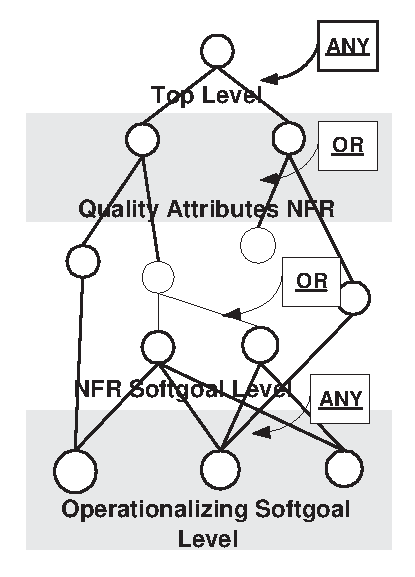
\includegraphics[width=1.5in]{fig/arch_def_loose_graph.eps}

\end{center}
\caption{logic configuration for weak quality assurance scheme}
\label{fig:arch_def_loose_graph}
\end{figure}

\begin{table}[h]
 \begin{footnotesize} 
 \begin{center}
 \begin{tabular}[t]{|c|c@{ }c@{ }c@{ }c@{ }c@{ }c|c|} \hline
 & \multicolumn{6}{c|}{Benefit} & \\ 
Cost	&$<14.67$ 	& $<29.33$ 	& $<44$ 	& $<58.67$ 	& $<73.33$ 	& $<87$	& \\ \hline
0	&	 	& 	 	& 	 	& 	 	& 	 	& 	 	& 	 \\
1	& \sq{3.06}{96} 	& 	 	& 	 	& 	 	& 	 	& 	 	& \sq{3.06}{96} \\
2	& \sq{6.99}{93} 	& \sq{10.36}{89} 	& \sq{0.62}{99} 	& \sq{0.02}{99} 	& 	 	& 	 	& \sq{17.99}{82} \\
3	& \sq{4.18}{95} 	& \sq{25.26}{74} 	& \sq{11.92}{88} 	& \sq{1.41}{98} 	& \sq{0.1}{99} 	& 	 	& \sq{42.87}{57} \\
4	& \sq{1.72}{98} 	& \sq{12.88}{87} 	& \sq{13.26}{86} 	& \sq{3.61}{96} 	& \sq{0.31}{99} 	& \sq{0.04}{99} 	& \sq{31.82}{68} \\
5	& \sq{0.27}{99} 	& \sq{1.57}{98} 	& \sq{1.77}{98} 	& \sq{0.59}{99} 	& \sq{0.06}{99} 	& 	 	& \sq{4.26}{95} \\ \hline
total	& \sq{16.22}{83} 	& \sq{50.07}{49} 	& \sq{27.57}{72} 	& \sq{5.63}{94} 	& \sq{0.47}{99} 	& \sq{0.04}{99} 	& \sq{100}{2} \\ \hline

 \end{tabular}
 \end{center}
 \end{footnotesize}
 \caption{\textbf{Round 1} Percentage distributions of $benefit$s and $cost$s seen in 10,000 runs of fig \ref{fig:arch_def_loose_graph}; (weak quality assurance) no treatment}
 \label{arch_def_loose_worse4_1}

 \begin{footnotesize} 
 \begin{center}
 \begin{tabular}[t]{|c|c@{ }c@{ }c@{ }c@{ }c@{ }c|c|} \hline
 & \multicolumn{6}{c|}{Benefit} & \\ 
Cost	& $<14.67$ 	& $<29.33$ 	& $<44$ 	& $<58.67$ 	& $<73.33$ 	& $<87$	& \\ \hline
0	& 	 	& 	 	& 	 	& 	 	& 	 	& 	 	& 	 \\
1	& \sq{12.34}{87} 	& \sq{0.02}{99} 	& 	 	& 	 	& 	 	& 	 	& \sq{12.36}{87} \\
2	& \sq{9.18}{90} 	& \sq{18.66}{81} 	& \sq{1.77}{98} 	& \sq{0.05}{99} 	& 	 	& 	 	& \sq{29.66}{70} \\
3	& \sq{4.71}{95} 	& \sq{26.32}{73} 	& \sq{16.1}{83} 	& \sq{3.24}{96} 	& \sq{0.24}{99} 	& \sq{0.02}{99} 	& \sq{50.63}{49} \\
4	& \sq{0.5}{99} 	& \sq{3.29}{96} 	& \sq{2.8}{97} 	& \sq{0.7}{99} 	& \sq{0.06}{99} 	& 	 	& \sq{7.35}{92} \\
5	& 	 	& 	 	& 	 	& 	 	& 	 	& 	 	& 	 \\ \hline
total	& \sq{26.73}{73} 	& \sq{48.29}{51} 	& \sq{20.67}{79} 	& \sq{3.99}{96} 	& \sq{0.3}{99} 	& \sq{0.02}{99} 	& \sq{100}{2} \\ \hline
 \end{tabular}
 \end{center}
 \end{footnotesize}
 \caption{\textbf{Round 2} Constraints: $c4=yes$, $pipeAndFilter$ $of$ $targetSystem=no$  (weak quality assurance)}
 \label{arch_def_loose_worse4_2}


 \begin{footnotesize} 
 \begin{center}
 \begin{tabular}[t]{|c|c@{ }c@{ }c@{ }c@{ }c@{ }c|c|} \hline
 & \multicolumn{6}{c|}{Benefit} & \\ 
Cost	& $<14.67$ 	& $<29.33$ 	& $<44$ 	& $<58.67$ 	& $<73.33$ 	& $<87$	&\\ \hline
0	& 	 	& 	 	& 	 	& 	 	& 	 	& 	 	& 	 \\
1	& \sq{11.89}{88} 	& \sq{0.01}{99} 	& 	 	& 	 	& 	 	& 	 	& \sq{11.9}{88} \\
2	& \sq{9.03}{90} 	& \sq{18.6}{81} 	& \sq{1.95}{98} 	& \sq{0.04}{99} 	& 	 	& 	 	& \sq{29.62}{70} \\
3	& \sq{4.77}{95} 	& \sq{26.17}{73} 	& \sq{17.05}{82} 	& \sq{3.47}{96} 	& \sq{0.29}{99} 	& \sq{0.01}{99} 	& \sq{51.76}{48} \\
4	& \sq{0.38}{99} 	& \sq{2.77}{97} 	& \sq{2.91}{97} 	& \sq{0.56}{99} 	& \sq{0.1}{99} 	& 	 	& \sq{6.72}{93} \\
5	& 	 	& 	 	& 	 	& 	 	& 	 	& 	 	& 	 \\ \hline
total	& \sq{26.07}{73} 	& \sq{47.55}{52} 	& \sq{21.91}{78} 	& \sq{4.07}{95} 	& \sq{0.39}{99} 	& \sq{0.01}{99} 	& \sq{100}{2} \\ \hline
 \end{tabular}
 \end{center}
 \end{footnotesize}
 \caption{\textbf{Round 3} Constraints: $c3=yes$,$c4=yes$, $pipeAndFilter$ $of$ $targetSystem=no$  (weak quality assurance)}
 \label{arch_def_loose_worse4_3}

 \begin{footnotesize} 
 \begin{center}
 \begin{tabular}[t]{|c|c@{ }c@{ }c@{ }c@{ }c@{ }c|c|} \hline
 & \multicolumn{6}{c|}{Benefit} & \\ 
Cost	& $<14.67$ 	& $<29.33$ 	& $<44$ 	& $<58.67$ 	& $<73.33$ 	& $<87$	& \\ \hline
0	& 	 	& 	 	& 	 	& 	 	& 	 	& 	 	& 	 \\
1	& \sq{20.34}{79} 	& \sq{0.05}{99} 	& 	 	& 	 	& 	 	& 	 	& \sq{20.39}{79} \\
2	& \sq{8.38}{91} 	& \sq{28.29}{71} 	& \sq{4.62}{95} 	& \sq{0.18}{99} 	& 	 	& 	 	& \sq{41.47}{58} \\
3	& \sq{1.84}{98} 	& \sq{15.66}{84} 	& \sq{15.84}{84} 	& \sq{4.27}{95} 	& \sq{0.48}{99} 	& \sq{0.05}{99} 	& \sq{38.14}{61} \\
4	& 	 	& 	 	& 	 	& 	 	& 	 	& 	 	& 	 \\
5	& 	 	& 	 	& 	 	& 	 	& 	 	& 	 	& 	 \\ \hline
total	& \sq{30.56}{69} 	& \sq{44}{56} 	& \sq{20.46}{79} 	& \sq{4.45}{95} 	& \sq{0.48}{99} 	& \sq{0.05}{99} 	& \sq{100}{2} \\ \hline

 \end{tabular}
 \end{center}
 \end{footnotesize}
 \caption{\textbf{Round 4} Constraints: $c2=yes$,$c3=yes$,$c4=yes$, $pipeAndFilter$ $of$ $targetSystem=no$  (weak quality assurance)}
 \label{arch_def_loose_worse4_4}

 \end{table}

%\input{dart}

\begin{figure}[h]
\begin{center}
\includegraphics[width=3.5in]{fig/cara_analysis.ps}
\includegraphics[width=2in]{fig/test.ps}
\end{center}
\caption{Segment of the SR-1 framework}
\label{fig:cara_analysis_graph}
\end{figure}

\begin{figure}[h]
 \begin{footnotesize} 
 \begin{center}
 \begin{tabular}[t]{|l|c@{ }c@{ }c@{ }|c@{ }c@{ }c@{ }c|c|} \hline
 Function & \multicolumn{3}{|c|}{Criticality} & \multicolumn{4}{c|}{Risk} & \\ 
 	& Cr[a]  	&  Cr[b] 	 & Cr[c] 	&  Ri[a] 	& Ri[b] 	& Ri[c] 	& Ri[d] & Level \\ \hline
f[vm]	&4	&4	&2	&3	&2	&3	&3	&F \\
f[guid]	&4	&4	&2	&3	&2	&2	&3	&F \\
f[nav]	&4	&4	&2	&3	&2	&2	&3	&F \\
f[sFilter]	&4	&4	&2	&3	&1	&2	&3	&F \\
f[telem]	&4	&1	&3	&3	&1	&3	&2	&F \\
f[tFilter]	&4	&1	&2	&3	&2	&2	&3	&L \\
f[cont]	&4	&4	&1	&2	&1	&2	&1	&L \\
f[cam]	&2	&1	&1	&3	&3	&2	&3	&B \\
f[exInf]	&3	&2	&1	&1	&1	&2	&1	&N \\
f[oReqm]	&3	&3	&3	&1	&2	&2	&3	&F \\
f[sMode]	&3	&1	&3	&3	&2	&2	&3	&L \\
f[aMode]	&3	&1	&3	&3	&2	&2	&3	&L \\
f[tMode]	&3	&1	&3	&3	&2	&2	&3	&L \\
f[dMode]	&3	&1	&2	&3	&2	&2	&3	&L \\
f[sbMode]	&1	&3	&1	&1	&1	&2	&2	&L \\
f[pMode]	&3	&1	&1	&1	&1	&2	&2	&N \\
f[aexInf]	&3	&1	&1	&2	&1	&2	&1	&N \\
f[comm]	&3	&1	&1	&1	&1	&3	&1	&N \\  \hline
 \end{tabular}
 \end{center}
 \end{footnotesize}
 \caption{CARA ratings on SR-1 software functions and corresponding Analysis Level}
 \label{fig:cara_result}

\end{figure}

\newpage


\begin{figure}[h]

 \begin{footnotesize} 
 \begin{center}
 \begin{tabular}[t]{|l|c|c|} \hline
Code 	& Level & Cost \\ \hline
 \multicolumn{3}{|c|}{Requirements Analysis Activities} \\ \hline
 rav01	&B,L,F,C	&notHigh \\
rav02	&B,L,F,C	&notHigh \\
rav03	&B,L,F,C	&notHigh \\
rav04	&B,L,F,C	&notHigh \\
rav05	&B,L,F,C	&notHigh \\
rav06	&B,L,F,C	&notHigh \\
rav07	&B,L,F,C	&notHigh \\
rav08	&B,L,F,C	&notHigh \\
rav09	&B,L,F,C	&notHigh \\
rav10	&F,C	&veryHigh \\
rav11	&F,C	&veryHigh \\
rav12	&F,C	&veryHigh \\
rav13	&F,C	&veryHigh \\
rav14	&C	&extremelyHigh \\ \hline
 \multicolumn{3}{|c|}{Design Analysis Activities} \\ \hline
dav01	&L,F,C	&high\\
dav02	&L,F,C	&high\\
dav03	&L,F,C	&high\\
dav04	&L,F,C	&high\\
dav05	&L,F,C	&high\\
dav06	&L,F,C	&high\\
dav07	&L,F,C	&high\\
dav08	&L,F,C	&high\\
dav09	&L,F,C	&high\\
dav10	&F,C	&veryHigh\\
dav11	&F,C	&veryHigh\\
dav12	&F,C	&veryHigh\\
dav13	&F,C	&veryHigh\\
dav14	&C	&extremelyHigh\\ \hline
 \multicolumn{3}{|c|}{Code Analysis Activities} \\ \hline
cav01	&L,F,C	&high\\
cav02	&L,F,C	&high\\
cav03	&L,F,C	&high\\
cav04	&L,F,C	&high\\
cav05	&L,F,C	&high\\
cav06	&L,F,C	&high\\
cav07	&F,C	&veryHigh\\
cav08	&F,C	&veryHigh\\
cav09	&F,C	&veryHigh\\
cav10	&F,C	&veryHigh\\
cav11	&F,C	&veryHigh\\
cav12	&C	&extremelyHigh\\
cav13	&C	&extremelyHigh\\
cav14	&C	&extremelyHigh\\ \hline
 \multicolumn{3}{|c|}{Test Analysis Activities} \\ \hline
tav01	&B,L,F,C	&high\\
tav02	&B,L,F,C	&high\\
tav03	&B,L,F,C	&high\\
tav04	&B,L,F,C	&high\\
tav05	&B,L,F,C	&high\\
tav06	&B,L,F,C	&high\\
tav07	&B,L,F,C	&high\\
tav08	&L,F,C	&veryHigh\\
tav09	&L,F,C	&veryHigh\\
tav10	&F,C	&veryHigh\\
tav11	&F,C	&veryHigh\\
tav12	&C	&extremelyHigh\\ \hline
 \end{tabular}
 \end{center}
 \end{footnotesize}
 \caption{Analysis Activities, applicable Analysis Levels for SR-1's functions, and Cost}
 \label{fig:analysis_acivities}

\end{figure}

\newpage

\begin{figure}[h]
 \begin{tiny} 
 \begin{center}
 \begin{tabular}[t]{|l@{ }|l@{ }|} \hline
Code 	& Requirements Analysis Activity\\ \hline
Rav01	&Verify documentation meets intended purpose, has appropriate detail and all necessary elements. \\
Rav02	&Validate ability of requirements to meet system needs \\
Rav03	&Verify Traceability to and from parent requirements \\
Rav04	&Analyze data/adaptation requirement \\
Rav05	&Analyze Testability, Qualification requirements \\
Rav06	&Analyze Data FnotHigh, Control FnotHigh, moding and sequencing \\
Rav07	&Assess development metrics \\
Rav08	&Analyze development risks/mitigation plans \\
Rav09	&Analyze Timing and Sizing requirements \\
Rav10	&Review developer timing/sizing, loading engineering analysis \\
Rav11	&Perform engineering analysis of key algorithms \\
Rav12	&Review/use developer prototypes or dynamic models \\
Rav13	&Develop alternative static representations (diagrams, tables) \\ \hline

Code 	& Design Analysis Activity	\\  \hline
Dal01	&Verify documentation meets intended purpose, has appropriate detail and all necessary elements \\
Dal02	&Validate ability of design to meet system needs \\
Dal03	&Verify Traceability to and from requirements \\
Dal04	&Analyze database design \\
Dal05	&Analyze design Testability, Qualification requirements \\
Dal06	&Analyze design Data FnotHigh, Control FnotHigh, moding, sequencing \\
Dal07	&Analyze control logic, error/exception handling design \\
Dal08	&Assess design development metrics \\
Dal09	&Analyze development risks/mitigation plans \\
Dal10	&Review developer timing/sizing, loading engineering analysis \\
Dal11	&Perform design analysis of select critical algorithms \\
Dal12	&Review/use developer prototypes or dynamic models \\
Dal13	&Develop alternative static representations (diagrams, tables) \\

Code 	& Code Aalysis Activity	\\  \hline
Cal01	&Verify documentation meets intended purpose, has appropriate detail and all necessary elements \\
Cal02	&Verify Traceability to and from design \\
Cal03	&Verify Architectural design compliance  \\
	& (structure, external I/O, and CSCI executive moding, sequencing and control) \\
Cal04	&Verify supportability and maintainability \\
Cal05	&Access code static metrics \\
Cal06	&Verify CSU and CSC level logical structure and control fnotHigh \\
Cal07	&Verify internal data structures and data fnotHigh/usage \\
Cal08	&Verify error and exception handling \\
Cal09	&Verify code and external I/O data consistency \\
Cal10	&Verify correct adaptation data and ability to reconfigure \\
Cal11	&Verify correct operating system and run time libraries \\ \hline

Code 	& Test Analysis Activity	\\  \hline
Tal01	&Analyze System level verification requirements to verity that test definition, objectives, plans and  \\
	& acceptance criteria are sufficient to validate system requirements and operational needs  \\
	& associated with CCHR functions \\
Tal02	&Verify Software Test Plan qualification testing methods and plans are sufficient to validate software \\
	&  requirements and operational needs \\
Tal03	&Verify test cases traceability and coverage of software requirements, operational needs and capabilities \\
Tal04	&Verify software STD test case definition inputs, expected results, and evaluation criteria comply with \\ 
	& STP plans and testing objectives \\
Tal05	&Analyze correct dispositioning of software test anomalies \\
Tal06	&Validate software test results compliance with test acceptance criteria \\
Tal07	&Verify trace and successful completion of all software test case objectives \\
Tal08	&Verify ability of software test environment plans and designs to meet software testing objectives \\
Tal09	&Verify regression tests are sufficient to determine that the software is not adversely affected \\
	& by changes \\
Tal10	&Analyze STD procedures for test setup, execution, and data collection; confirm procedures completely  \\
	& and correctly test referenced requirements, confirm inspection and analysis completely verifies referenced  \\
	& requirements \\
Tal11	&Monitor execution of software testing as needed \\ \hline

 \end{tabular}
 \end{center}
 \end{tiny}
 \caption{Analysis Activities Keys to figure \ref{fig:analysis_acivities}}
 \label{fig:analysis_acivities_key}
 
\end{figure}

\begin{figure}[h]
\begin{center}
\begin{footnotesize}
 \begin{tabular}[t]{|l|c|c|} \hline
version 			& 1		& 2	\\ \hline
{\verb1<notHigh>1}	& $mean(X)=1$		& $mean(X)=$\\
($X$)		&			& $mean(Y)*0.7$	\\ \hline
{\verb1<high>1} 	& $Y=$			& $mean(Y)=2$, \\
($Y$)		& $mean(X)*10$		& $0<Y<10$\\ \hline
{\verb1<veryHigh>1}	&$Z=$		&$mean(Z)=Y*F$, \\
($Z$)		&$mean(Y)*10$	&$mean(F)=1.2$; $1.1\leq F \leq 1.7$ \\ \hline
 \end{tabular}
\end{footnotesize}
\end{center}
 \caption{Two versions of cost function}
\label{fig:cara_analysis_cost}
\end{figure} 

\begin{figure}[h]
\begin{center}
\begin{footnotesize}
 \begin{tabular}[t]{|c|c|c|} \hline
 {\verb1<combine_logic>1}		& {\verb1<op>1} 		& {\verb1<arithmetic[op]>1}\\ \hline
 {\sl all\_of}			& {\verb1rand1}		& minimum \\
 {\sl any\_of}			& {\verb1rany1}		& summation \\
 {\sl any\_one\_of}			& {\verb1ror1}		& maximum \\ \hline
 {\verb1<contribution>1}		& {\verb1<value>1} 	& {\verb1<arithmetic>1}\\ 
 				& {\verb1[contribution]1}	& {\verb1[contribution]1}\\ \hline
 {\sl helped}			& mean=1.4		& multiply \\
 {\sl made}			& mean=1.8		& multiply \\
 {\sl catastrophically\_rated}		& mean=1.9		& multiply \\
 {\sl critically\_rated}			& mean=1.4		& multiply \\
 {\sl highly\_rated}			& mean=1.1		& multiply \\
 {\sl lowly\_rated}			& mean=0.4		& multiply \\ \hline
 \end{tabular}
\end{footnotesize}
\end{center}
 \caption{Miscellaneous settings for SR-1 framework}
\label{fig:cara_analysis_config}
\end{figure} 



 \begin{table}[h]
 \begin{center}
 \begin{small}
 \begin{tabular}[t]{|c|cccc|} \hline
 & \multicolumn{4}{c|}{Benefit} \\ 
 Cost	& vlow 	& low 	& high 	& vhigh	\\ \hline
 vlow 	& 10 	& 5 	& 2 	& 1 	\\ 
 low 	& 12	& 7 	& 4 	& 3 	\\ 
 high 	& 14 	& 9 	& 8 	& 6 	\\ 
 vhigh 	& 16 	& 15 	& 13 	& 11 	\\ \hline
 \end{tabular}
 \end{small}
 \end{center}
 \caption{class rankings for SR-1 framework}
 \label{tab:cara_analysis}
 \end{table}

\begin{figure}[h]
\begin{center}
 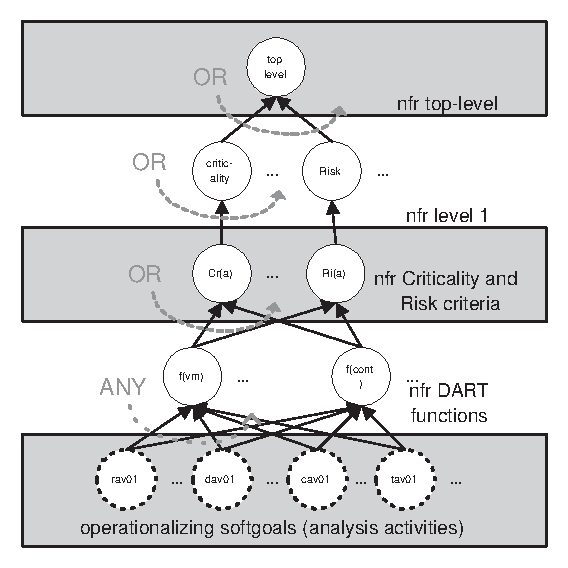
\includegraphics[width=3in]{fig/or3a.eps}

\end{center}
\caption{SR-1 framework: 1}
\label{fig:cara_analysis_or3any}

\end{figure}

\begin{figure}[h]
\begin{center}
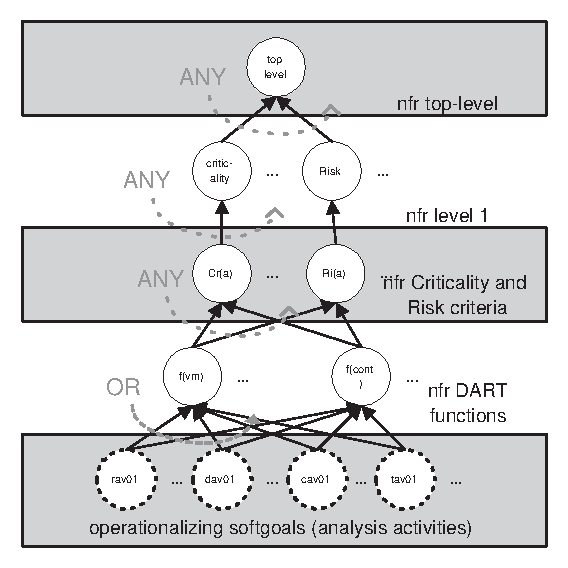
\includegraphics[width=3in]{fig/any3or.eps}

\end{center}
\caption{SR-1 framework: 2}
\label{fig:cara_analysis_any3or}
\end{figure}

\begin{figure}[h]
\begin{center}
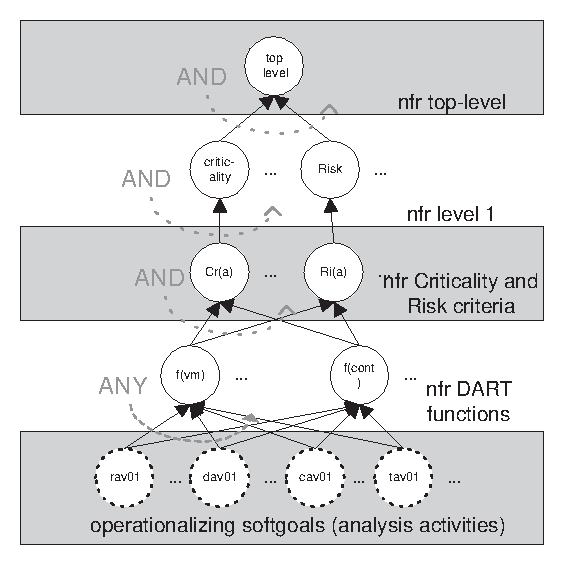
\includegraphics[width=3in]{fig/and3any.eps}

\end{center}
\caption{SR-1 framework: 3}
\label{fig:cara_analysis_and3any}
\end{figure}

%%%% or3any %%%%%%%%%
\begin{table}[h]
 \begin{footnotesize} 
 \begin{center}
 \begin{tabular}[t]{|c|c@{ }c@{ }c@{ }c|c|} \hline
 & \multicolumn{4}{c|}{Benefit} & \\ 
 Cost	& vlow		& low		& high	& vhigh		& Total	\\ \hline
vlow 	& \sq{34.15}{66} 	& 	 	& 	 	& 	 	& \sq{34.15}{66} \\
low 	& 	 	& \sq{4.02}{96} 	& \sq{6.26}{94} 	& \sq{5.58}{95} 	& \sq{15.86}{85} \\
high 	& 	 	& \sq{6.2}{94} 	& \sq{9.98}{91} 	& \sq{8.82}{92} 	& \sq{25}{75} \\
vhigh 	& 	 	& \sq{5.64}{95} 	& \sq{8.76}{92} 	& \sq{10.59}{90} 	& \sq{24.99}{76} \\
Total 	& \sq{34.15}{66} 	& \sq{15.86}{85} 	& \sq{25}{75} 	& \sq{24.99}{76} 	& \sq{100}{2} \\ \hline
 \end{tabular}
 \end{center}
 \end{footnotesize}
 \caption{\textbf{SR-1 framework 1}  
 Percentage distributions of $benefit$s and $cost$s seen in 10,000 runs of fig \ref{fig:cara_analysis_or3any}; no treatment}
 \label{cara_analysis_or3any_noT}

 \begin{footnotesize} 
 \begin{center}
 \begin{tabular}[t]{|c|c@{ }c@{ }c@{ }c|c|} \hline
 & \multicolumn{4}{c|}{Benefit} & \\ 
 Cost	& vlow		& low		& high	& vhigh		& Total	\\ \hline
vlow 		& 		& 		& 		& 		& 	\\
low	& 		& \sq{4.70}{96} 	& \sq{7.74}{93} 	& \sq{7.30}{93} 	& \sq{19.7}{81} \\
high	& 		& \sq{9.95}{91} 	& \sq{16.0}{84} 	& \sq{14.2}{86} 	& \sq{40.1}{60} \\
vhigh	& 		& \sq{9.05}{91} 	& \sq{14.1}{86} 	& \sq{17.0}{83} 	& \sq{40.1}{60} \\
total	& 		& \sq{23.7}{77} 	& \sq{37.8}{63} 	& \sq{38.5}{62} 	& \sq{100}{2} \\ \hline
 \end{tabular}
 \end{center}
 \end{footnotesize}
 \caption{\textbf{More preferred system: SR-1 framework 1}  
 Percentage distributions of $benefit$s and $cost$s seen after applying treatments ($tav09$ $of$ $tal=y$) for a more desirable system}
 \label{cara_analysis_or3any_B}
 
 \begin{footnotesize} 
 \begin{center}
 \begin{tabular}[t]{|c|c@{ }c@{ }c@{ }c|c|} \hline
 & \multicolumn{4}{c|}{Benefit} & \\ 
 Cost	& vlow		& low		& high	& vhigh		& Total	\\ \hline
vlow	& 	 	& 	 	& 	 	& 	 	& 	 \\
low	& 	 	& 	 	& 	 	& 	 	& 	 \\
high	& 	 	& \sq{5.16}{95} 	& \sq{9.52}{91} 	& \sq{8.6}{92} 	& \sq{23.27}{77} \\
vhigh	& 	 	& \sq{17.32}{83} 	& \sq{26.9}{74} 	& \sq{32.51}{68} 	& \sq{76.73}{24} \\
Total	& 	 	& \sq{22.47}{78} 	& \sq{36.41}{64} 	& \sq{41.11}{59} 	& \sq{100}{2} \\ \hline
 \end{tabular}
 \end{center}
 \end{footnotesize}
 \caption{\textbf{Less preferred system: SR-1 framework 1}  
 Percentage distributions of $benefit$s and $cost$s seen after applying treatments ($cav10$ $of$ $cal=y$) for a less desirable system}
 \label{cara_analysis_or3any_W}
 
\end{table}

%%%% any3or %%%%%%%%%
\begin{table}[h]
 \begin{footnotesize} 
 \begin{center}
 \begin{tabular}[t]{|c|c@{ }c@{ }c@{ }c|c|} \hline
 & \multicolumn{4}{c|}{Benefit} & \\ 
 Cost	& vlow	& low	& high	& vhigh	& Total\\ \hline
vlow	& \sq{17.63}{83} 	& \sq{2.21}{98} 	& \sq{2.67}{98} 	& \sq{2.5}{98} 	& \sq{25.01}{75} \\
low	& \sq{3.84}{97} 	& \sq{8.76}{92} 	& \sq{6.16}{94} 	& \sq{6.24}{94} 	& \sq{25}{75} \\
high	& \sq{2.48}{98} 	& \sq{8}{92} 	& \sq{7.12}{93} 	& \sq{7.4}{93} 	& \sq{25}{75} \\
vhigh	& \sq{1.06}{99} 	& \sq{6.03}{94} 	& \sq{9.05}{91} 	& \sq{8.85}{92} 	& \sq{24.99}{76} \\
Total	& \sq{25.01}{75} 	& \sq{25}{75} 	& \sq{25}{75} 	& \sq{24.99}{76} 	& \sq{100}{2} \\ \hline

 \end{tabular}
 \end{center}
 \end{footnotesize}
 \caption{\textbf{SR-1 framework 2}  
 Percentage distributions of $benefit$s and $cost$s seen in 10,000 runs of fig \ref{fig:cara_analysis_any3or}; no treatment}
 \label{cara_analysis_any3or_noT}

 \begin{footnotesize} 
 \begin{center}
 \begin{tabular}[t]{|c|c@{ }c@{ }c@{ }c|c|} \hline
 	& \multicolumn{4}{c|}{Benefit} 	& \\ 
 Cost	& vlow	& low	& high	& vhigh	& Total\\ \hline
vlow	& \sq{25.35}{75} 	& \sq{3.13}{97} 	& \sq{3.83}{97} 	& \sq{3.6}{97} 	& \sq{35.91}{65} \\
low	& \sq{4.88}{96} 	& \sq{11.58}{89} 	& \sq{8.4}{92} 	& \sq{8.66}{92} 	& \sq{33.52}{67} \\
high	& \sq{2.26}{98} 	& \sq{7.65}{93} 	& \sq{6.67}{94} 	& \sq{7.61}{93} 	& \sq{24.19}{76} \\
vhigh	&  	& \sq{1.56}{99} 	& \sq{2.16}{98} 	& \sq{2.32}{98} 	& \sq{6.38}{94} \\
Total	& \sq{32.84}{68} 	& \sq{23.91}{77} 	& \sq{21.06}{79} 	& \sq{22.18}{78} 	& \sq{100}{2} \\ \hline
 \end{tabular}
 \end{center}
 \end{footnotesize}
 \caption{\textbf{More preferred system: SR-1 framework 2}  
 Percentage distributions of $benefit$s and $cost$s seen after applying treatments ($dav12$ $of$ $dal=n$) for a more desirable system}
 \label{cara_analysis_any3or_B}
 
 \begin{footnotesize} 
 \begin{center}
 \begin{tabular}[t]{|c|c@{ }c@{ }c@{ }c|c|} \hline
 	& \multicolumn{4}{c|}{Benefit} 	& \\ 
 Cost	& vlow	& low	& high	& vhigh	& Total\\ \hline
vlow	&  	&  	& 	 	& 	 	&  \\
low	& \sq{3.4}{97} 	& \sq{5.69}{95} 	& \sq{1.65}{99} 	& \sq{2.11}{98} 	& \sq{12.86}{88} \\
high	& \sq{5.51}{95} 	& \sq{15.52}{85} 	& \sq{7.71}{93} 	& \sq{6.98}{94} 	& \sq{35.72}{65} \\
vhigh	& \sq{4.13}{96} 	& \sq{12.95}{88} 	& \sq{16.71}{84} 	& \sq{17.17}{83} 	& \sq{50.96}{50} \\
Total	& \sq{13.22}{87} 	& \sq{34.44}{66} 	& \sq{26.08}{74} 	& \sq{26.26}{74} 	& \sq{100}{2} \\ \hline
 \end{tabular}
 \end{center}
 \end{footnotesize}
 \caption{\textbf{Less preferred system: SR-1 framework 2}  
 Percentage distributions of $benefit$s and $cost$s seen after applying treatments ($cav07$ $of$ $cal=y$) for a less desirable system}
 \label{cara_analysis_any3or_W}
 
\end{table}

% ----------------------------------------------------------------------------------------------------------- %
%\section{Conclusion and Future Work}
% ----------------------------------------------------------------------------------------------------------- %

%conclude here

\newpage

%%%%%%%%%%%%%%%%%%%%%%%%%%%%%%%%%%%%%%%
%\bibliographystyle{plain}
%\bibliography{cfp}

%%%%%%%%%%%%%%%%%%%%%%%%%%%%%%%%%%%%%%%

\newpage
% ----------------------------------------------------------------------------------------------------------- %


%\bibliographystyle{abbrv}
%\bibliographystyle{IEEE}
%{\footnotesize \bibliography{cfp}}

%\appendix

%\input{mm}

\newpage



% ----------------------------------------------------------------------------------------------------------- %

\end{document}